\documentclass[a4paper,11pt]{article}
\usepackage[utf8]{inputenc}
\usepackage[english]{babel}
\usepackage[top=2cm, bottom=2cm, left=3cm, right=3cm]{geometry}
\usepackage[onehalfspacing]{setspace}
\usepackage{amsmath,xcolor,graphicx,hyperref}
\usepackage[charter]{mathdesign}

\hypersetup{
	colorlinks=true,
	linkcolor=black,
	urlcolor=blue,
	citecolor=black
}

\author{
	\emph{Prof.: Marco Maffezzoli}
	\and
	\emph{TA: Andrea Pasqualini}%
		\thanks{
			Author of this document.
			Comments are welcome: \href{mailto:andrea.pasqualini@phd.unibocconi.it}{andrea.pasqualini@phd.unibocconi.it}.
		}
}

\title{
	\textbf{Macroeconomics 3} \\
	TA session 1, Exercise set
}

\date{
	PhD in Economics and Finance, A.y.~2017-2018 \\
	Bocconi University, Milan
}

\begin{document}
	\maketitle

	This is a set of exercises to get you started with Python and the modules \texttt{numpy} and \texttt{matplotlib}.
	\textbf{No hand-in required}.
	For every exercise, there is more than one way to obtain the intended result, so experimenting is encouraged.
	The first seven exercises are simply intended to warm you up with Python (they're silly, I know), while the others are a bit more serious and focused on what we will do.
	If you have questions, feel free to ask me.

	\begin{enumerate} \setcounter{enumi}{-1}
		\item
			Create a dictionary with the name of 4/5 students and years of birth and derive a list with the ages by using a list comprehension.
			Obtain also a new dictionary with the same keys as the original containing the ages computed above.
		
		\item
			Define a function \texttt{myMax()} that takes two numbers as arguments and returns the largest of them, and complains if the type of inputs is incorrect.
		
		\item
			Write a function that takes a character (i.e., a string of length 1) and returns True if it is a vowel, False otherwise.
			\emph{[Extra: validate your inputs, i.e., check for unsuitable inputs]}
		
		\item
			Write a function that takes a list and returns a new list that contains all the elements of the original list without duplicates (if any).
			\emph{[Extra: validate your inputs]}
		
		\item
			Write a function that computes the dot product of two given lists leveraging the zip() function.
			\emph{[Extra: validate your inputs]}
		
		\item
			Write a recursive function \texttt{fibonacci(n)} that returns the $n$-th element of the Fibonacci series.
		
		\item
			Enclose the answer to the previous exercise into a \texttt{Class} that you will call \texttt{Fibonacci}.
			This class should have two methods: \texttt{element} and \texttt{series}.
			\texttt{Fibonacci.element(n)} will return only the $n$-th element of the series, while \texttt{Fibonacci.series(n)} will return a tuple (not a list!) that consists of the Fibonacci sequence up to the $n$-th entry. \\
			\emph{[Hint: remember that Python starts counting from zero]} \\
			\emph{[Extra: validate your inputs]}
		
		\item
			Suppose a certain Markov Chain has the following right-stochastic transition matrix:
			\begin{align*}
				\Pi &=
				\begin{bmatrix}
					0.2 & 0.8 \\
					0.7 & 0.3
				\end{bmatrix}
			\end{align*}
			Create the matrix using \texttt{numpy} and compute the $N$-step ahead transition matrix for some arbitrary $N$.
			\emph{Extras:}
			\begin{enumerate}
				\item \emph{write code that simulates the markov chain;}
				\item \emph{write code that finds the stationary distribution;}
				\item \emph{write everything using a class, with input validation, i.e., $\Pi$ must be a square matrix and right-stochastic.}
			\end{enumerate}
			\emph{[Hint: Google is your best friend]}

		\item
			Suppose that you want to evaluate a polynomial $p(x)$ defined as
			\begin{align*}
				p(x) &= a_0 + a_1 x + a_2 x^2 + \ldots + a_{n-1} x^{n-1} \\
						 &= \sum_{i=0}^{n-1} a_i x^i.
			\end{align*}
			You do not want to choose a value $x$ necessarily.
			Therefore, write a \texttt{Class} that, for a given \texttt{tuple} or \texttt{list} $a$:
			\begin{itemize}
				\item has a method that evaluates $p(x)$ at a given $x_0$;
				\item has a method that computes the first derivative of $p(x)$ at a given $x_0$;
				\item plots the function in a given domain.
			\end{itemize}
			You can only use the following external help: \texttt{from numpy import array, linspace} and \texttt{from matplotlib.pyplot import subplots}
		
		\item 
			Let $X = [0,1] \subset \mathbb{R}$ and consider the function $f : X \to X$ such that
			\begin{align*}
				f(x) &= \sqrt{1+x} - \dfrac{2}{3},
					& x \in X.
			\end{align*}
			As you know, we can construct a sequence ${(x_n)}_{n=0}^{\infty}$ through the iteration $x_{n+1} = f(x_n)$, given an initial condition $x_0$.
			The sequence so obtained is convergent because $f$ is a contraction.
			The limit is the fixed point of the contraction.

			Write some code that implements the iteration and finds the fixed point: start from an arbitrary initial condition $x_0$ and stop when $x_{n+1}$ and $x_n$ are ``close enough.''
			Keep track of the (finite) sequence ${(x_n)}_{n=0}^{N-1}$ visited by the algorithm.
			You can only use the following import statement: \texttt{from numpy import sqrt, array}. 
			\emph{[Extra: define a function that performs the iteration for a given ``function handle'' and initial condition]}

		\item 
			Using the answer to the previous exercise and the path converging to the fixed point you obtained with the iterative algorithm, replicate \emph{exactly} Figure \ref{fig:fixed_point}.%
				\footnote{
					\emph{Exactly} means that you must replicate the figure in every single detail, including the absence of the box around the graph, the order in which the lines have been drawn, the text written with \LaTeX, the width of the lines, the size of the overall figure, etc.
				}
			The original figure is a PDF file 5 inches wide and 4 inches tall.
			You can use anything that you find useful in \texttt{numpy} and \texttt{matplotlib}.
			\emph{[Hint: Google is your best friend]}
			\begin{figure}
				\centering
				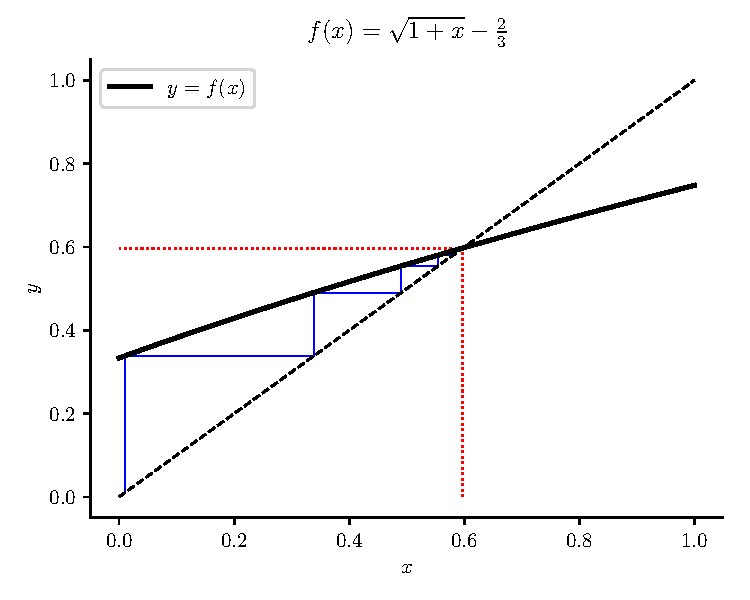
\includegraphics{./fixed_point.pdf}
				\caption{Path visited by the algorithm $x_{n+1} = f(x_n)$ and location of the fixed point.
				The initial condition is $x_0 = 0.01$.}
				\label{fig:fixed_point}
			\end{figure}
	\end{enumerate}
\end{document}
